
%!TEX root = paper.tex
We collected ratings from the Movielens users on certain groups of movies. These
groups were generated by selecting five movies from the movies that the user has
already rated. There was no overlap among the groups presented to the user in a
session. The user can rate at most 50 such groups in a session. An example of
the questionnaire eliciting a user's rating on a group of movies is shown in the
Figure~\ref{fig:mlset}. The rating widget in the interface could be rated from 0 to 5 with a
precision of 0.5.

\begin{figure}[ht]
  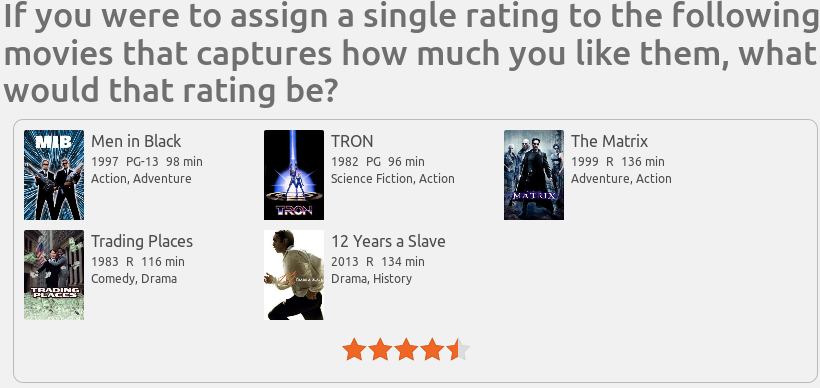
\includegraphics[scale=0.30]{figures/mlset.png}
  \caption{The interface used to elicit users' ratings on a group of movies.}
  \label{fig:mlset}
\end{figure}


Before processing the dataset, we removed users who have rated groups within a
time interval of less than one second to avoid users who might be guessing
ratings at random. After this pre-processing step, we were left with ratings
from 854 users over 29,516  sets containing 12,549 items. The
Figure~\ref{fig:setratingdist} depicts
the distribution of the collected ratings. We also computed the mean rating of
each user and is shown in the Figure~\ref{fig:meanratingdist}.  

\begin{figure}[ht]
  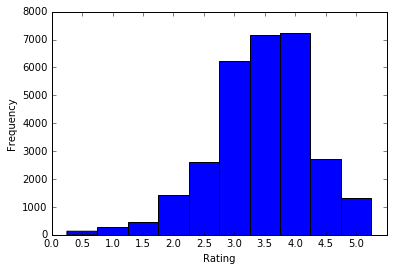
\includegraphics[scale=0.65]{figures/setratingdist.png}
  \caption{Ratings distribution.}
  \label{fig:setratingdist}
\end{figure}

\begin{figure}[ht]
  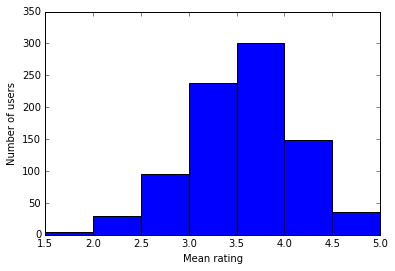
\includegraphics[scale=0.65]{figures/meanratingdist.png}
  \caption{The distribution of users' mean rating.}
  \label{fig:meanratingdist}
\end{figure}



The Figure~\ref{fig:usergroupdist} shows the distribution of the number of groups rated by the user,
and we can see that roughly half of the users, i.e., 428 users have rated more
than 90\% of the groups, i.e., at least 45 groups in a session.

\begin{figure}[ht]
  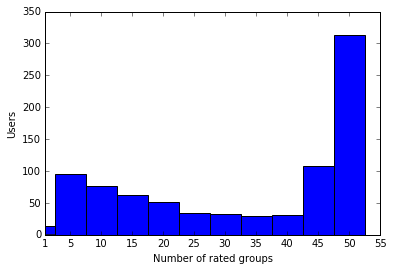
\includegraphics[scale=0.65]{figures/usergroupdist.png}
  \caption{The distribution of number of groups rated by the users.}
  \label{fig:usergroupdist}
\end{figure}


